
\chapter{The ATLAS Inner Tracker}
\label{chap:itk}
% This chapter highlights aspects of the ITk:
% \begin{enumerate}
%     \item Technical spec
%     \item Simulation (drawn from TDR)
%     \item Anything else that we need for subsequent chapters
% \end{enumerate}
The Inner Tracker (ITk) is the successor to the current Inner Detector (ID) in the High-Luminosity era.
It inherits many design features from the Pixel and SCT components of the ID, but with significant improvements in granularity, geometry coverage, material budget and expected parameter resolution. 
Understanding of its geometry and interaction with charged particles is crucial to fully simulate its detector response, extract useful information from track candidates, and interpret tracking results.
In this chapter describes aspects of the ITk design and simulation, providing a foundation for the discussion in subsequent chapters. 

\section{Overview of the Inner Tracker}
\label{sect:itk-overview}

The Inner Tracker consists of two silicon-based sub-detectors, a Pixel Detector close to the interaction point (IP) and a Strip Detector at a larger radius, and, unlike the Inner Detector, without the Transition Radiation Tracker. 
They feature a total area of $180$ $\mathrm{m}^2$ with more than 5 billion readout channels, in comparison to $63$ $\mathrm{m}^2$ and 100 million channels in the ID, translating to a significant increase in granularity. 
In the barrel region, the pixel subsystem comprises five layers and the strip subsystem four layers.
Each of the endcaps is equipped with six strip rings with petal design and many thin pixel rings. 
The layout of the ITk, demonstrated in figure \ref{fig:itk-layout}, is optimized to provide maximal hit coverage across the pseudorapidity range. 

\begin{figure}[h]
    \begin{subfigure}[b]{0.49\textwidth}
        \centering
        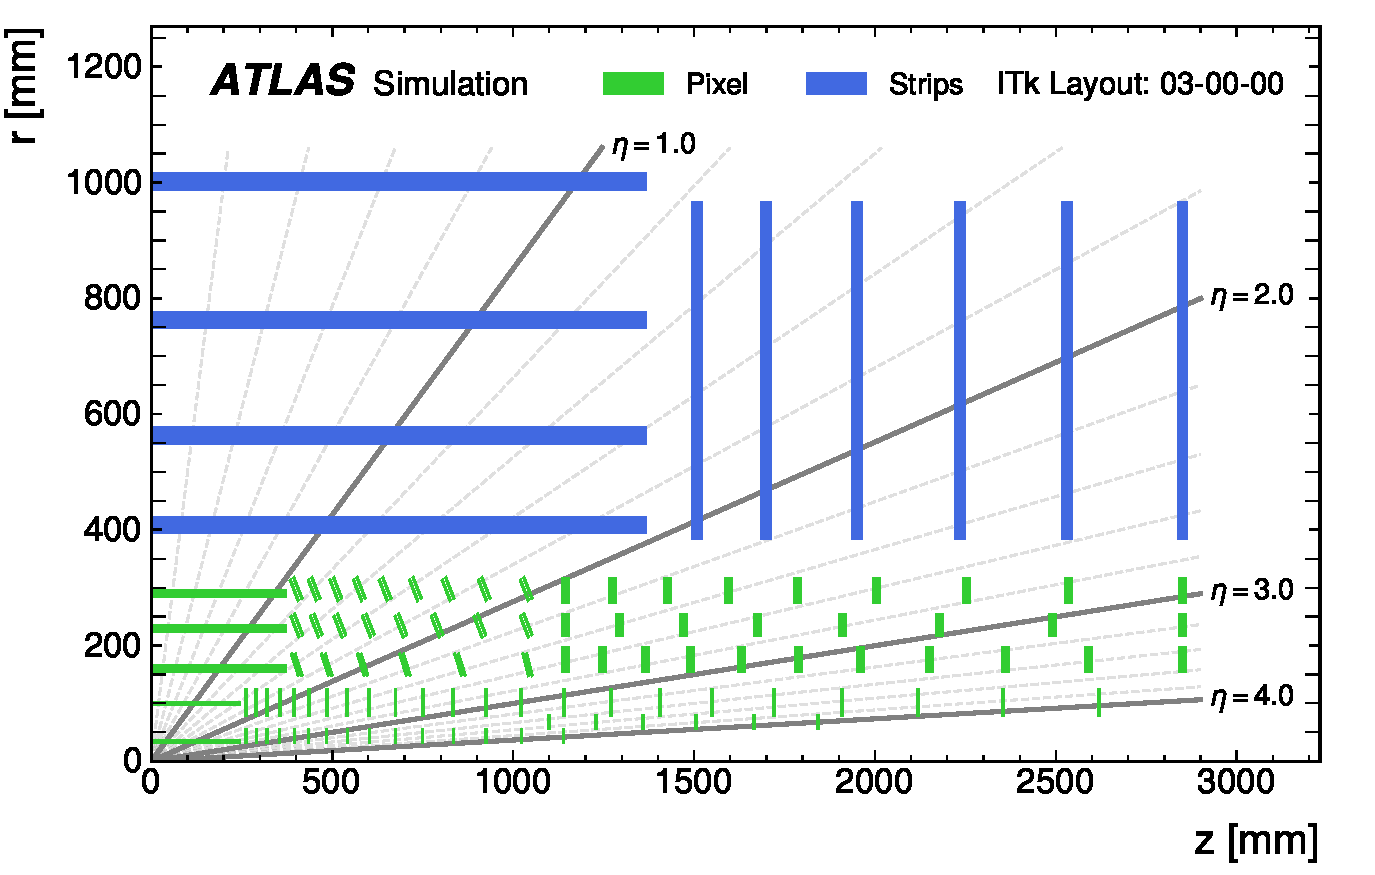
\includegraphics[width=\linewidth]{figures/itk-layout.pdf}
        \caption{}
        \label{subfig:itk-layout}
    \end{subfigure}
    \begin{subfigure}[b]{0.49\textwidth}
        \centering
        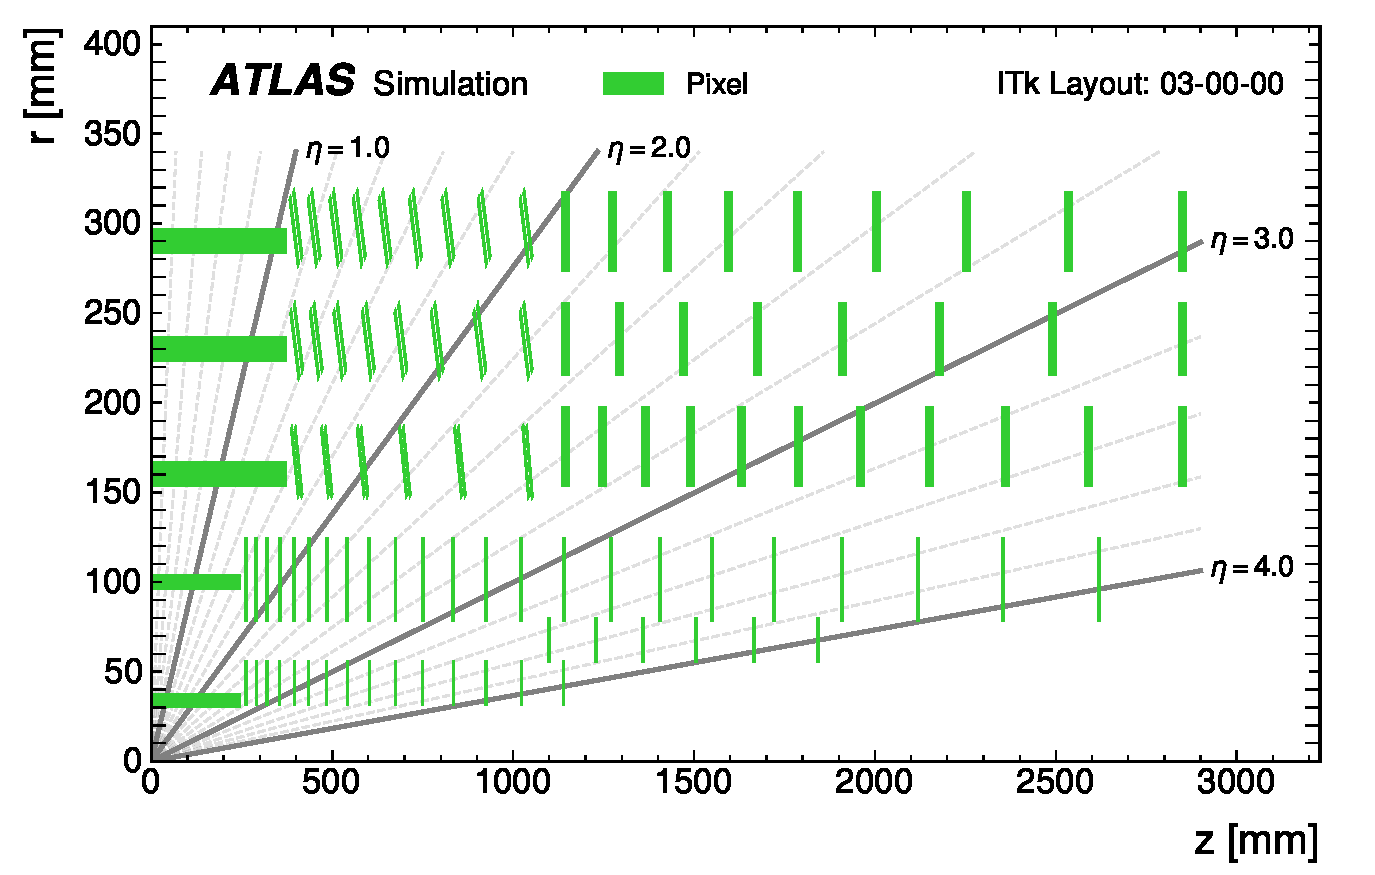
\includegraphics[width=\linewidth]{figures/itk-layout-pixel.pdf}
        \caption{}
        \label{subfig:itk-layout-pixel}
    \end{subfigure}
    \caption{A schematic view of the ITk layout (a), and of the pixel detector layout (b), both in one quadrant. Only active elements are visible in both figures. Pixel and strip elements are respectively shown in green and blue. The IP is located at the origin. The horizontal axis is parallel to the beam line, and the vertical axis is the radius measured from the IP~\cite{Aad_2025}.}
    \label{fig:itk-layout}
\end{figure}

The ITk is immersed in a solenoidal magnetic field of 2T, whose principal component lies largely along the $z$-axis. 
The bending power of the magnetic field creates a curvature in the trajectory of a charged particle, from which its transverse momentum $p_T$ is deduced. 
In addition, the ITk produces tracking measurements in close proximity to the IP, which plays an important role in impact parameter estimation, vertex fitting and subsequent pile-up mitigation.
In addition, the detector is designed to measure at least 9 hits per track in the barrel region and 13 in the endcaps, which provide strong constraints on the curvature of the track. 
Finally, pseudorapidity coverage is extended up to $\abs{\eta}=4$, in comparison to $\abs{\eta}<2.5$ in the ID. 

The ITk layout plays an important role in simulation and event reconstruction. 
It has undergone numerous refinements and evolutions since the first layout detailed in the technical design reports \cite{ATLAS-TDR-25, ATLAS-TDR-30}, with the current edition designated 03-00-00. 
All subsequent results in this document are evaluated on data simulated using this version. 

The pixel system is divided into three subsystems: the Inner System, the Outer Barrel, and the Outer Endcap. 
The Inner System (IS) encompasses the two innermost layers of the pixel detector, the first of which is located at a radius of 34 mm from the beam pipe. 
Because of its proximity to the luminous region, the IS is exposed to the highest radiation damage of the entire ITk, and is thus designed to be replaced after 2000 $\ifb$ of data has been recorded, when its modules are anticipated to deteriorate. 
The Outer Barrel (OB) radially covers the IS in the central region at larger radii, and consists of three layers of modules and three sets of endcap rings. 
As seen on figure \ref{subfig:itk-layout-pixel}, the inner rings of the OB are mounted at an incline angle to maximize the angular coverage while using less silicon, and to minimize the material length traversed by a particle having $1.0<\abs{\eta}<2.8$. 
The third subsystem, the Outer End-cap (OE), contains three sets of double-sided rings located on each side of the OB at $\abs{z}\approx 3000$ mm.

The pixel detector uses two different types of silicon sensors, namely 3D and planar sensors, depending on the radiation dose expected at different layers. 
The former is installed on the innermost layer and rings of the IS due to its radiation hardness, which is improved with respect to the 3D sensors employed in the ID. 
The rest of the pixel layers and rings uses planar sensors. 
The dimension of a pixel featured on the 3D sensor is 25 $\mu m$ in $R\phi$ direction and 100 $\mu m$ in the longitudinal direction, while the rest of the detector uses $50\times 50$ $\mu m^2$ pixels. 
The small pixel size implies a better resolved cluster shape, and subsequently improves impact parameter resolution. 
The pixel detector layout in the barrel and endcaps is summarized in tables \ref{tab:pixel-barrel-inclined-rings} and \ref{tab:pixel-endcap-rings}. 
In both tables, the triplet module features three connected read-out chips each processing electronic signals from a $2\times 2\, \mathrm{cm}^2$ sensor, and the quad module features 4 connected chips processing signals from a single $4\times4\,\mathrm{cm}^2$ sensor. 

\begin{table}[h]
    \centering
    \scalebox{0.9}{
    \begin{tabular}{|c|c|c|c|c|c|c|c|c|}
    \hline
        Barrel & Radius  & Rows of  & Flat barrel  & Incl. rings  & Incl.  & Module  & Sensor  & Sensor\\
        layer & [mm]  & sensors  & $\abs{z}$ [mm] & per row  & $\abs{z}$ [mm] & ring  & type  & dim. $[\mu \mathrm{m}^2]$ \\ \hline
        0 & 34 & 12 & 0-245 & 24 &  &  & triplets & $25\times100$\\
        1 & 99 & 20 & 0-245 & 12 &  &  & quads & $50\times50$\\
        2 & 160 & 32 & 0-372 & 18 & 380-1035 & $2\times6$ & quads & $50\times50$\\
        3 & 228 & 44 & 0-372 & 18 & 380-1035 & $2\times8$ & quads & $50\times50$\\
        4 & 291 & 56 & 0-372 & 18 & 380-1035 & $2\times9$ & quads & $50\times50$\\
        \hline
    \end{tabular}
    }
    \caption{Representative parameters of the pixel flat barrel and inclined rings in the ITk layout 03-00-00. Note that while all pixel layers have rings, only the OB features inclined rings. The fifth column provides the number of flat sensors mounted on a complete stave in the central barrel of each layer. The number of inclined rings is given by 2 $\times$ the number of rings on each of the barrel~\cite{Aad_2025}.}
    \label{tab:pixel-barrel-inclined-rings}
\end{table}

\begin{table}[h]
    \centering
    
    \begin{tabular}{|c|c|c|c|c|c|c|}
    \hline
        Ring & Radius  & $\abs{z}$ & Rings        & Sensors  & Module   & Sensor  \\
        layer& [mm]    & [mm]      &              & per ring & type     & dim. $[\mu\mathrm{m}^2]$ \\ \hline
        0    & 33.20   & 263-1142  & $2\times 15$ & 18       & triplets & $50\times50$\\
        0.5  & 58.70   & 1103-1846  & $2\times 6$ & 30       & triplets & $50\times50$\\
        1    & 80.00   & 263-2621  & $2\times 23$ & 20       & quads    & $50\times50$\\
        2    & 154.50  & 1145.5-2850  & $2\times 11$ & 32       & quads    & $50\times50$\\
        3    & 214.50  & 1145.5-2850  & $2\times 8$ & 44       & quads    & $50\times50$\\
        4    & 274.60  & 1145.5-2850  & $2\times 9$ & 52       & quads    & $50\times50$\\
        \hline
    \end{tabular}
    \caption{Representative parameters of the pixel endcaps in the ITk layout 03-00-00. The radius in the second column refers to the radius of the circle formed by the innermost point of the sensors on each ring. The number of rings is twice the number of rings on each of the barrel~\cite{Aad_2025}.}
    \label{tab:pixel-endcap-rings}
\end{table}

The strip detector is divided into two subsystems: the barrel region and two endcap regions with different arrangements of sensor modules. 
Figure \ref{fig:strip-stave-petal} shows an overview of the support structure and the arrangement of strip modules in each subsystem. 
In the barrel region, four cylindrical barrel layers surround the beam line and cover $\abs{z} < 1.4$ m. 
Each layer consists of staves running parallel to the $z$-axis, on each side of which 14 modules are mounted. 
The strips on each side of the stave are rotated with respect to the $z$-axis by $\pm26$ mrad to form a stereo angle of 52 mrad between the microstrip on the two sides. 
Since each microstrip provides a one-dimensional measurement, the stereo angle allows an estimate of a second coordinate from combining the measurements on both side of the stave. 
The strips on the two inner cylinders are 24.1 mm long and those on the outer two are 48.2 mm long, designated respectively as short- and long-strips. 
The barrel sensors are tilted in the $R\phi$ plane to allow for an overlap between neighbouring sensors which ensures detection coverage over the entire azimuthal range ($\phi$-hermeticity). 
Table \ref{tab:strip-barrel} shows the number of staves, tilt angle, and strip length on each barrel strip layer. 

\begin{figure}[h]
    \centering
    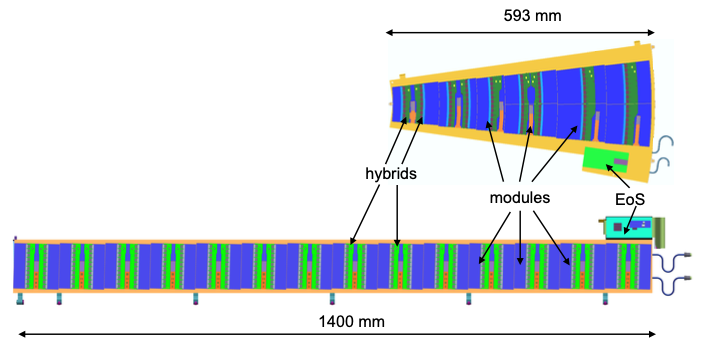
\includegraphics[width=0.8\linewidth]{figures/strip-stave-petal.png}
    \caption{Overview of the endcap petal (upper) and barrel stave (lower) in the strip detector. Sensor modules shown in blue are mounted directly on a rigid carbon-fiber sandwich structure. Only one half of a stave is shown~\cite{ATLAS-TDR-25}.}
    \label{fig:strip-stave-petal}
\end{figure}

The endcap region features six disks on each side, the outermost of which is located at $\abs{z}=3$ m. Each endcap disk is partitioned into 32 identical wedge-shaped petals, and each petal contains nine modules on each side organized into six subsegments referred to as rings (figure \ref{fig:strip-stave-petal}). The strips on each side are constructed with a stereo angle of $\pm20$ mrad with respect to the radial line that bisects the petal, achieving a total stereo angle of 40 mrad between the two sides. Because of the increasing circumferences of the petal rings, each of them has a distinct sensor geometry and electronic arrangement. These features are detailed in the Technical Design Report~\cite{ATLAS-TDR-25}.

\begin{table}[h]
    \centering
    \begin{tabular}{|c|c|c|c|c|}
    \hline
       Barrel  & Number of & Radius [mm] & Tilt           & Strip \\
       layer   & staves    &             & angle [degree] & length [mm] \\ \hline
        0      & 56         & 399 & 13 &  2.5 \\
        1       & 80        & 562 & 12 &  2.5 \\
        2       & 112       & 762 & 12 &  5 \\
        3       & 144       & 1000 & 11 & 5 \\ \hline
    \end{tabular}
    \caption{Characterization of the strip barrel, including the number of staves, radius, tilt angle, and strip length in the ITk layout 03-00-00~\cite{Aad_2025}.}
    \label{tab:strip-barrel}
\end{table}

\section{Simulation of the Inner Tracker}
\label{sect:itk-simulation}
The production of data samples used to study track reconstruction in the ITk proceeds through several steps: event generation, detector simulation using \GEANT \cite{Agostinelli:2002hh}, and digitization of simulated energy deposits. 
% The last step in the chain is the reconstruction of charged-particle tracks from the digitized data. In offline tracking, the reconstruction step is carried out by an algorithm called the Combinatorial Kalman Filter (CKF). The purpose of this work is finding a candidate replacement for the CKF which scales better under HL-LHC pile-up condition. 
Detector simulation is the costliest and the most difficult step, having to account for complex detector effects on the particle's trajectory.
Charged particles interact with the material through which they travel via several mechanisms. 
Because material interactions can change both the magnitude and direction of particle momentum, an accurate description of the material distribution in the detector is crucial to the modelling of particle trajectories as well as the extraction of track parameters from track candidates. 
Particular care was taken to describe the material at a high level of detail. 
The dimensions, location, and material of all detector elements are implemented in the simulation framework. 
The location of the material is shown in figure \ref{fig:itk-material-location}. 
The materials are defined in \GEANT in terms of their chemical composition and density.

\begin{figure}[h!]
    \centering
    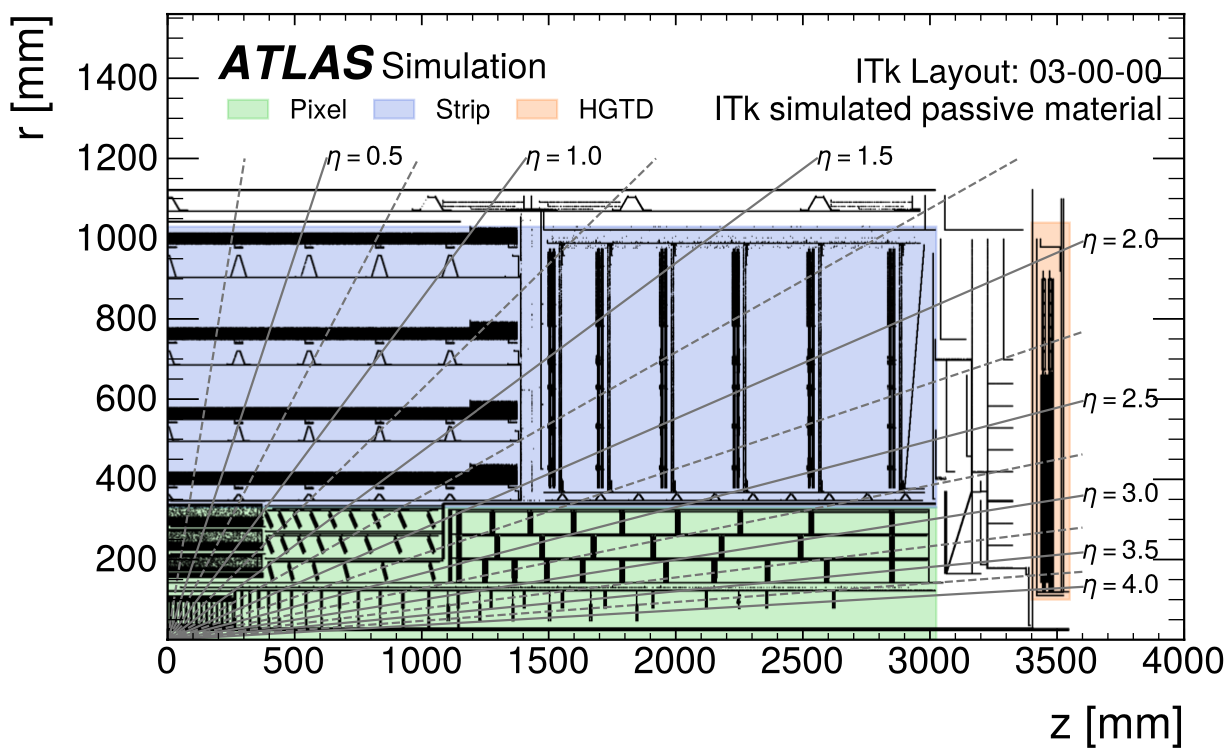
\includegraphics[width=0.75\linewidth]{figures/itk-material-location.png}
    \caption{Location of the materials for one quadrant of the ITk layout 03-00-00. The pixel subsystem is shown in green and surrounded by the strip subsystem shown in blue. The location of the materials are indicated by black regions~\cite{2HDMWGproxi}. }
    \label{fig:itk-material-location}
\end{figure}

\subsection{Simulation of the Pixel Detector }

The Pixel Detector is divided into a barrel region and two identical endcaps. The outer barrel support structure is modelled using the longeron support structure, shown in figure \ref{fig:itk-longeron}. The longeron truss structures are approximated as thin sheets of carbon fiber, and the main rails supporting the truss, accounting for 80\% of the mass, are modelled by denser materials. 

The inner barrel support structure is modelled as truss double shells, with one shell per layer. The shells are modelled as a sheet of carbon fiber behind each row of modules. The total mass of each shell in the support structure is adjusted to match the corresponding engineering estimate. The outer pixel endcaps are modelled as rings. Each layer of rings is also supported by a cylindrical carbon-fiber shell.

\begin{figure}[h!]
    \centering
    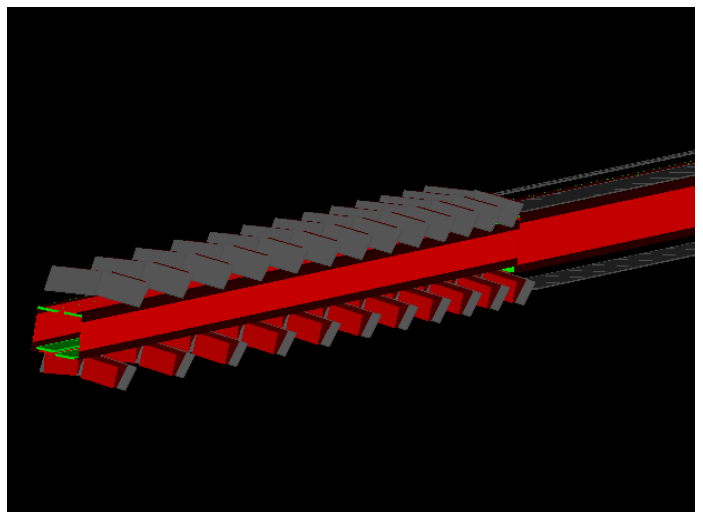
\includegraphics[width=0.5\linewidth]{figures/itk-longeron.png}
    \caption{An illustration of the \GEANT geometry model of the outer barrel longeron stave with mounted inclined and flat modules. Figure taken from reference~\cite{ATLAS-TDR-30}.}
    \label{fig:itk-longeron}
\end{figure}

Pixel modules are modelled as an active sensor volume and a front-end (FE) chip. Layer 0 of both the barrel in the endcaps features 3D pixel sensors. The active part of the sensor is implemented as a 150-$\mu m$ thick layer of silicon and the support wafer as a 100-$\mu m$ thick layer of inactive silicon. Other layers feature planar pixel sensors, modelled as 100-$\mu m$ and 150-$\mu m$ thick active silicon respectively in layer 1 and layers 2-4. 

Front-end chips are modelled as a 150-$\mu m$ thick silicon wafer, with a 1-$\mu$m thick copper layer to model its circuitry, and a Sn-Ag bump bond of 20-$\mu$m in diameter per pixel channel. The material of each component in the FE chips is homogeneously distributed throughout its corresponding volume.

\subsection{Simulation of the Strip Detector}

In the strip barrel detector, each individual part is modelled separately, with masses and material compositions reflecting the mechanical designs. In the strip endcaps, materials and objects in close proximity with each other are not individually modelled, but instead as one homogeneous block of material adjusted to have the same radiation length as calculated based on engineering designs. Figure \ref{fig:itk-strip} displays the \GEANT  geometry model of barrel staves and endcap petals in the Strip detector. 

\begin{figure}[h!]
    \begin{subfigure}[b]{0.49\textwidth}
        \centering
        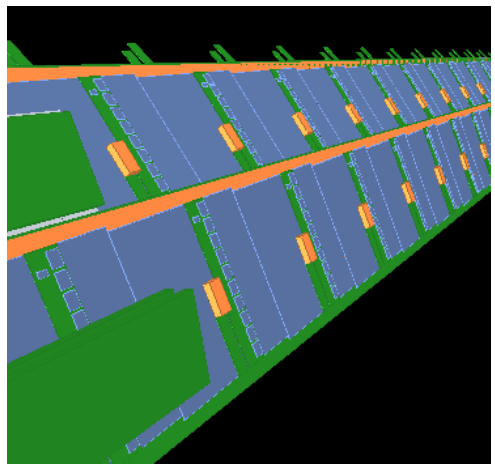
\includegraphics[width=\textwidth]{figures/itk-barrel-staves.png}
        \caption{}
        \label{subfig:itk-barrel-staves}
    \end{subfigure}
    \begin{subfigure}[b]{0.49\textwidth}
        \centering
        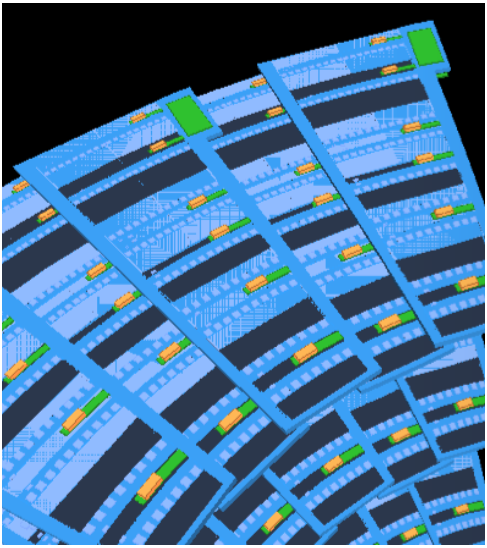
\includegraphics[width=\textwidth]{figures/itk-endcap-petals.png}
        \caption{}
        \label{subfig:itk-endcap-petal}
    \end{subfigure}
    \caption{Displays of the \GEANT geometry model of the strip barrel staves (left) and the endcap petals (right). Figure taken from reference~\cite{ATLAS-TDR-30}.}
    \label{fig:itk-strip}
\end{figure}

The global support of the detector in both the barrel and the endcaps is modelled in detail. Components include stave cooling pipes, carbon-foam, facesheets, cable bus, hybrids, and FE ASICs. Endcap sensors are individually modelled, while other components are modelled as a single edge-shaped object sandwiched between two silicon layers and uniformly filled with a generic material. The density of the material is adjusted to provide a radiation length of 0.02 $X_0$ per substructure. 

\section{Particle interaction with detector material}
\label{sect:material-effects}

An important aspect of realistic detector simulation as well as track reconstruction is the treatment of interactions between high-energy particles and the materials they traverse. 
For charged particles at the energy range relevant to the Inner Tracker, these interactions are dominated by two processes: (i) inelastic collisions with atomic electrons, and (ii) elastic scattering against atomic nuclei. 
In turn, they result in two primary effects: (1) a loss in energy by the particle, and (2) a deflection from the original direction of incident.  
Of the two electromagnetic processes, inelastic collisions are responsible for the greater part of the energy loss from heavy particles in matter. 
Each collision transfers but a tiny fraction of the particle's energy to the incident atom, causing an ionization or excitation of the latter\footnote{To demonstrate the scale of each energy loss, note that atomic excitations are often measured in eV, while particle energy is often given in MeV or GeV.}. 
However, the number of collisions encountered by a particle per unit path length in dense materials is typically large enough that a non-negligible amount of its energy is lost to the environment. 

\subsection{Energy loss of heavy particles}\label{subsect:e-loss-heavy}

The probability of an inelastic collision is described by the quantum mechanical scattering amplitude calculated for the corresponding process. 
In a macroscopic path length, a particle undergoes so many collisions that the distribution of total energy loss sharply peaks around an average value. 
Therefore, it is sufficient to compute the average energy loss per unit length, also called the stopping power or $\frac{dE}{dx}$. 
The stopping power of a material on an incident particle in the momentum range relevant to the ITk is given by the Bethe-Bloch formula \cite{Zyla:2020zbs}
\begin{equation}
    \label{eq:6.1}
    -\frac{dE}{dx} = 2\pi N_a r_e^2 m_e c^2 \frac{Z}{A} \left( \frac{z^2}{\beta^2}\right) \left[ \log \left( \frac{2m_e \gamma^2 v^2 W_{max}}{I^2}\right) - 2\beta^2 -\delta   \right],
\end{equation}
in which $r_e = 2.817\times 10^{-13}$ cm is the classical electron radius, $m_e$ the electron mass, $N_a$ the Avogadro's number, $I$ the mean excitation potential, $Z$ and $A$ the atomic number and atomic weight of the absorbing material, $z$ the charge of the incident particle in units of $e$, $\beta $ the $\frac{v}{c}$ ratio, $\gamma = (1-\beta^2)^{-1/2}$ the usual relativistic $\gamma$ factor, $\delta$ the density correction, and $W_{max}$ the maximum energy transfer in a single collision.
% \begin{itemize}
%     \item $r_e = 2.817\times 10^{-13}$ cm: classical electron radius, 
%     \item $m_e$: electron mass
%     \item $N_a$: Avogadro's number
%     \item $I$: mean excitation potential
%     \item $Z$: atomic number of absorbing material
%     \item $A$: atomic weight of absorbing material 
%     % \item $\rho$: density of absorbing material 
%     \item $z$: charge of the incident particle in $e$
%     \item $\beta $ : $\frac{v}{c}$ ratio of the particle 
%     \item $\gamma = (1-\beta^2)^{-1/2}$
%     \item $\delta$: density correction 
%     \item $W_{max}$: maximum energy transfer in a single collision.
% \end{itemize}
The maximum energy transfer depends on the ratio of the electron mass and the particle mass
\begin{equation}
    \label{eq:6.2}
    W_{max} = \frac{2m_ec^2\beta^2\gamma^2}{1+2\gamma (m_e/M) + (m_e/M)^2}.
\end{equation}
The left hand size of equation \eqref{eq:6.1} is called the mass stopping power, which varies slowly with different materials. The average energy loss per unit length is simply given by $\rho \left(  \frac{dE}{dx}\right)$. Shown in figure \ref{fig:bethe-bloch} is the mass stopping power computed for a positive muon in copper over 12 order of magnitude in muon momentum. The region corresponding to $10$ MeV $<p_{\mu ^+}< $ 100 GeV, most relevant in high-energy physics, is called the Bethe region where the stopping power is a function of $\beta$ alone. At non-relativistic energies, $\frac{dE}{dx}$ is dominated by the overall $1/\beta^2$ factor (note the logarithmic scale in the vertical axis of \ref{fig:bethe-bloch}). The stopping power reaches a minimum at $\beta\gamma\approx 3$, and slowly rises thanks to the logarithmic dependence up to $\beta\gamma = 1000$, a range equivalent to a muon momentum of $1-100$ GeV. This minimum is broad and almost the same for all particles of the same charge. For this reason, particles at this point are called ``minimum-ionizing".  
\begin{figure}[h!]
    \centering
    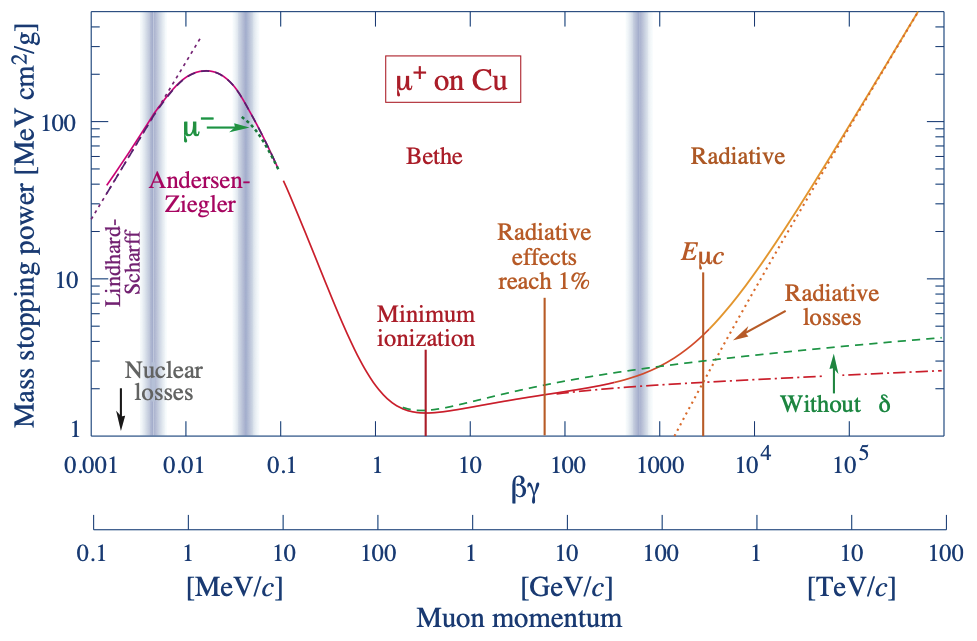
\includegraphics[width=0.9\linewidth]{figures/bethe-bloch.png}
    \caption{The mass stopping power of positive muons in copper as a function of the muon momentum spanning nine orders of magnitude. The solid curves indicate the total stopping power of all dissipative effects. The region of interest in HEP ranges from 100 MeV to 100 GeV, well within the so-called Bethe region, in which the stopping power is strongly dependent on $\beta$ (see text for definition). Figure taken from reference~\cite{Zyla:2020zbs}.}
    \label{fig:bethe-bloch}
\end{figure}

The stopping power in equation \eqref{eq:6.1} is computed for pure elements. A non-elemental material can be considered as a mixture of elements, whose stopping power is approximated by a weighted mean of $\frac{dE}{dx}$ over the elements in the compound. The weight is given by the fraction of electrons contributed by each element. In particular, the average mass stopping power is
\begin{equation}
    \label{eq:6.3}
    \frac{dE}{dx} = \sum_i w_i\left( \frac{dE}{dx} \right)_i, \quad \quad w_i = \frac{a_i A_i}{\sum_j a_j A_j}
\end{equation}
where $a_i$ is the number of atoms in the $i$-th element, and $A_i$ the atomic weight. Knowing the stopping power of each element in a material and the molecular composition, one can easily compute the mean energy loss of an incident particle given its momentum. 

Because of the statistical nature of inelastic collisions, the amount of energy deposited by a particle fluctuates around the mean calculated in equation \eqref{eq:6.1}. 
In a relatively thick absorber, the number of collisions is large, and, assuming each collision results in a small energy loss $\delta E$, such that the particle velocity stays constant, the stopping power $\frac{dE}{dx}$ negligibly varies throughout the particle's path.
The total energy loss is thus the sum of a large number of independent identically distributed random energy losses, which approaches a Gaussian as $N\rightarrow \infty$
\begin{equation}
    \label{eq:6.4}
    f(\Delta E; x) = \frac{1}{\sqrt{2\pi}\sigma } \exp \left[ \frac{-(\Delta E - \expval{\Delta E})^2}{2\sigma ^2} \right], \quad\quad \expval{\Delta E} = \int_0 ^ {x} \left(\frac{dE}{dx'} \right)dx'.
\end{equation}
with variance 
\begin{equation}
    \label{eq:6.5}
    \sigma = 0.1569 \rho \left( \frac{Z}{A} \right) \frac{1-\beta^2/2}{1-\beta^2} x.
\end{equation}

\subsection{Energy loss of electrons and positrons}
\label{subsect:e-loss-electron}
Light charged particles such as electrons and positrons undergo collisional energy loss in matter, just like heavy particles. However, because of their small mass, electromagnetic radiation in the electric field of atomic nuclei becomes a significant contribution to their overall rate of energy loss
\begin{equation}
    \label{eq:6.6}
    \left ( \frac{dE}{dx} \right) = \left ( \frac{dE}{dx} \right)_{rad} + \left ( \frac{dE}{dx} \right) _{col},
\end{equation}
in which $\left ( \frac{dE}{dx} \right)_{rad}$ is the radiative component and $\left ( \frac{dE}{dx} \right) _{col}$ the collisional component already described.

Even though the mechanism of collisional loss remains the same, because their mass is small, light particles could get deflected significantly from the original direction of incident. 
In addition, the collision occurs between identical particles, so several modifications to the Bethe equation are needed, starting with the maximum energy transfer $W_{max} = T/2$ where $T$ is the kinetic energy of the incident particle. The collisional stopping potential becomes
\begin{equation}
    \label{eq:6.7}
    -\left( \frac{dE}{dx}\right)_{col} = 2\pi N_a r_e^2 m_e c^2 \frac{Z}{A} \left( \frac{1}{\beta^2} \right) \left[ \log \frac{\tau^2 (\tau +2)}{2(I/m_ec^2)^2} + F(\tau) -\delta \right], \quad \quad \tau = \frac{T}{m_e c^2}
\end{equation}
where the function $F(\tau)$ modifies the $\beta^2$ term in equation \eqref{eq:6.1} to account for the interaction between identical particles, resulting from crossing Feynman diagrams:
$$
    F_{e^-}(\tau) = 1-\beta^2 + \frac{\tau^2 / 8 - (2\tau +1)\ln 2}{(\tau +1 )^2},
$$
and 
$$
    F_{e^+}(\tau) = 2\ln 2 - \frac{\beta^2}{12}\left( 23 + \frac{14}{\tau+2} + \frac{10}{(\tau+2)^2} + \frac{4}{(\tau + 2)^3} \right).
$$

Qualitatively, the radiative cross-section of bremsstrahlung is proportional to the inverse square of particle mass. Therefore, being far lighter than any other particle, electrons and, to a much lesser extent, muons lose a significant portion of their energy to this phenomenon. The radiative contribution to the mass stopping power can be written as
\begin{equation}
    \label{eq:6.8}
    -\left( \frac{dE}{dx}\right)_{rad} = \frac{N_a}{A}E\Phi_{rad},
\end{equation}
where $\Phi_{rad}$ is the total radiative cross section, approximated by 
\begin{equation}
    \label{eq:6.9}
    \Phi_{rad} = 4Z^2(e^2/m_ec^2)^2\alpha^2 \left [ \ln (183Z^{-1/3} ) + \frac{1}{18} - f(Z) \right],
\end{equation}
where $f(Z)$ is a small correction to the Born approximation accounting for the Coulomb interaction between the electron and the nucleus. 

It is straightforward to compare the two contributions of the total stopping power. Figure \ref{fig:rad-vs-col} demonstrates the the radiation and collisional energy losses for electron in copper as functions of the electron energy. Bremsstrahlung takes effect starting at 15 MeV, and at energy above a critical value of $\approx 25$ MeV, its contribution quickly dominates the total energy loss. This observation is due to the fact that collisional loss rises logarithmically with energy, whereas radiative loss scales linearly, evidenced by equations \eqref{eq:6.7} and \eqref{eq:6.8}. In the energy range from $1-100$ GeV relevant to the ITk, the electron stopping power is composed almost entirely of radiative loss. 

\begin{figure}[h!]
    \centering
    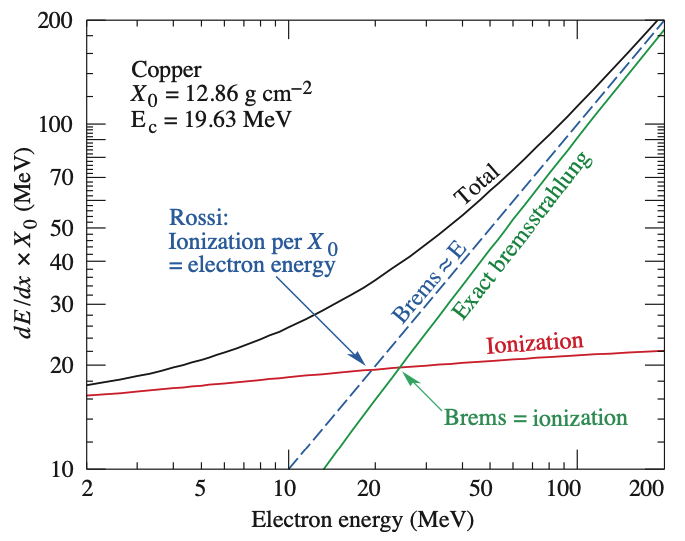
\includegraphics[width=0.65\linewidth]{figures/rad-vs-col.png}
    \caption{Contribution of radiative and collisional components in the total energy loss of electrons in copper as functions of electron energy. At a critical value $E_c=19.63$ MeV, radiative loss becomes the dominant mechanism. The energy range of electrons in HEP detectors is well within the Bremsstrahlung regime.}
    \label{fig:rad-vs-col}
\end{figure}
The critical energy at which the both components contribute equality to the total energy loss for a material is approximated by 
\begin{equation}
    \label{eq:6.10}
    E_c \,(\mathrm{MeV}) = \frac{800}{Z+1.2}
\end{equation}

It is evident that the material energy loss of electrons and positrons is characterized by the Bremsstrahlung cross section. 
In practice, it is more convenient to characterize a material by its radiation length $X_0$, defined as the distance over which the average electron energy is reduced by a factor of $1/e$ due to radiation loss. 
Equation \eqref{eq:6.8} can be rewritten as 
\begin{equation}
    \label{6.11}
    - \rho\left( \frac{dE}{dx}\right)_{rad} \frac{1}{E} = \frac{N_a\rho}{A} \Phi_{rad} = N\Phi_{rad} = \frac{1}{X_0}
\end{equation}
or 
\begin{equation}
    \label{eq:6.12}
    \boxed{E = E_0 \exp\left( -\frac{x}{X_0} \right)},
\end{equation}
where $N$ is the volumetric density of atomic nuclei in the material.

In the ITk, material thickness is described in units of radiation length. 
Figure \ref{subfig:itk-rad-len} shows the material thickness traversed by a straight track as a function of its pseudorapidity. 
Obviously, charged particles move in mostly helical orbits, whose curvature depends on the transverse momentum, because of the magnetic field, and thus the actual material length traversed by the particle is obtained by numerical integration. 
The central region has very little material, resulting from the light design of the sensor support. 
At higher $\eta$, a particle travels through progressively more layers and thus experiences almost linearly increasing material thickness. 
The largest contribution to the total radiation length comes from pixel services and cooling.

For comparison, the material depth of the ID in Run 2, including the Pixel, SCT and TRT, is shown in figure \ref{subfig:id-rad-len}, and expected material thickness traversed by a particle until it reaches the minimum number of hits required for track reconstruction in figure \ref{subfig:rad-len-to-reco}. 
The linear ITk material budget is significantly smaller than that of the ID in the forward region, despite having more layers and better eta coverage. 
This is due to the adoption of serial powering in the ITk, among other design optimizations. 
A realistic particle experiences up to 50\% more material before reaching the minimum number of hits for $\eta<1.5$ in the ITk than in the ID. 
Note, however that ID tracks are required to have only 8 hits in this region, compared to 9 hits for an ITk track. 
Beyond this point, the ITk becomes more transparent than the ID, by up to 50\%. 

\begin{figure}[h!]
\begin{subfigure}[b]{0.47\textwidth}
    \centering
    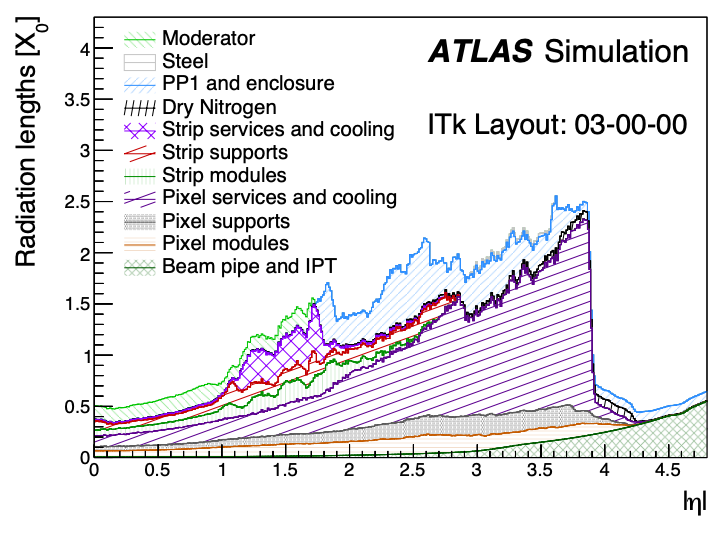
\includegraphics[width=\textwidth]{figures/itk-rad-length.png}
    \caption{ITk radiation length~\cite{Aad_2025}}
    \label{subfig:itk-rad-len}
\end{subfigure}
\begin{subfigure}[b]{0.51\textwidth}
    \centering
    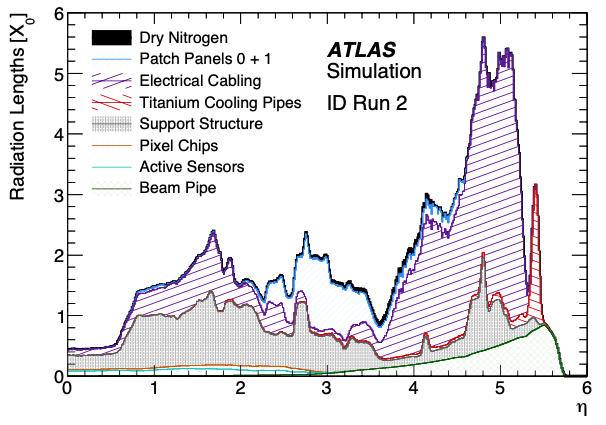
\includegraphics[width=\textwidth]{figures/id-rad-length.png}
    \caption{ID radiation length \cite{ATLAS-TDR-25}}
    \label{subfig:id-rad-len}
\end{subfigure}
\begin{subfigure}[b]{\textwidth}
    \centering
    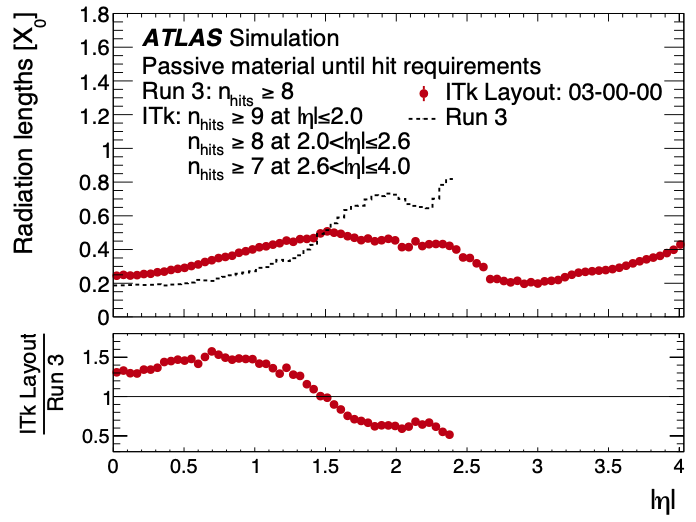
\includegraphics[width=0.5\textwidth]{figures/rad-length-to-reconstruct.png}
    \caption{Radiation length to reach reconstructible number of hits~\cite{Aad_2025}}
    \label{subfig:rad-len-to-reco}
\end{subfigure}
    \caption{Integrated material budget encountered on a particle's path in unit of radiation length as a function of pseudorapidity based on (a) the ITk and (b) the ID. The particle assumes a straight trajectory from the origin. (c) is a comparison between the amount of material that must be traverse before the particle accumulates enough hits to be deemed reconstructible.}
    \label{fig:rad-len}
\end{figure}

% A full simulation of particle trajectories takes into account the spatial material distribution and the initial value of particle momentum. The mean energy loss is numerically integrated from 
\subsection{Multiple Coulomb scattering}\label{subsect:multi-scat}

In addition to inelastic collision and radiation, charged particles undergo a large number of small-angle elastic scattering due to Coulomb interaction with atomic nuclei. 
Coulomb scatterings are governed by the Rutherford formula for non-relativistic collision, and the Mott formula for the relativistic counterpart. 
In both formulae, the scattering cross-section follows 
\begin{equation}
    \label{eq:6.13}
    \frac{d\sigma}{d\Omega} \propto \frac{1}{\sin^4 (\theta/2)}
\end{equation}
which favours a small scattering angle $\theta$. Assuming the material is sufficiently thick and the energy transfer to the nuclei is negligible, the particle suffers a large number of small deflections.
The net effect can therefore be statistically represented by a probability distribution function of the total deflection which depends on the material thickness. 
A rigorous treatment of multiple scattering is complicated. 
Among the most commonly used approximations is the theory of Molière \cite{Moliere:1947, Moliere:1948zz}, valid for the scattering of fast charged particles. 
The theory was expanded by Bethe~\cite{bethe:1953} and later Scott~\cite{scott:1963} to account for Coulomb interactions with atomic electrons. 
Although it agrees well with data, especially at small angles and large target nuclear numbers, it relies on an unwieldy series expansion and is therefore inconvenient to use. 
Rossi and Greisen~\cite{Rossi_Greisen_1941} developed a simple estimate of the root-mean-square scattering angle, which was improved by Highland~\cite{Highland_1975} and Lynch and Dahl~\cite{Lynch_Dahl_1991} to obtain the RSM width of the projected scattering angle distribution on a plane
\begin{equation}
\label{eq:6.14}
    \theta_0 = \frac{13.6z\, \mathrm{MeV}}{pc\beta} \sqrt{\frac{x}{X_0}}\left[ 1 + 0.038\ln \frac{z^2(x/X_0)}{\beta^2} \right],
\end{equation}
where $p$, $\beta c$, and $z$ are the momentum, the velocity, and the charge of the incident particle. $x/X_0$ is the material thickness in radiation lengths. 
The scattering angle projected on a plane $\theta_{plane}$ can be approximated by a Gaussian centered at $\theta_{plane}=0$
\begin{equation}
    \label{eq:6.15}
    d P(\theta_{plane}) = \frac{1}{\sqrt{2\pi} \theta_0} \exp \left[ - \frac{\theta_{plane}^2}{2\theta_0^2} \right] d\theta_{plane}
\end{equation}
The total angle $\vartheta$ can be approximated by the quadratic sum of two small projected angles on orthogonal planes
\begin{equation}
\label{eq:6.16}
\vartheta^2 = \theta_{plane,x}^2 + \theta_{plane,y}^2, \quad\quad d\vartheta = d\theta_{plane,x}d\theta_{plane,y}
\end{equation}
and with the assumption that the two projected angles are independent, $\vartheta_{tot}$ is 
\begin{equation}
\label{eq:6.17}
d P(\vartheta) = \frac{1}{2\pi \theta_0^2} \exp \left[ - \frac{\vartheta^2}{2\theta_0^2} \right] d\vartheta
\end{equation}
Figure \ref{fig:multi-scat} illustrates the quantities used to describe the effect of multiple scattering. The total scattering angle is projected on a plane 

\begin{figure}[h!]
    \centering
    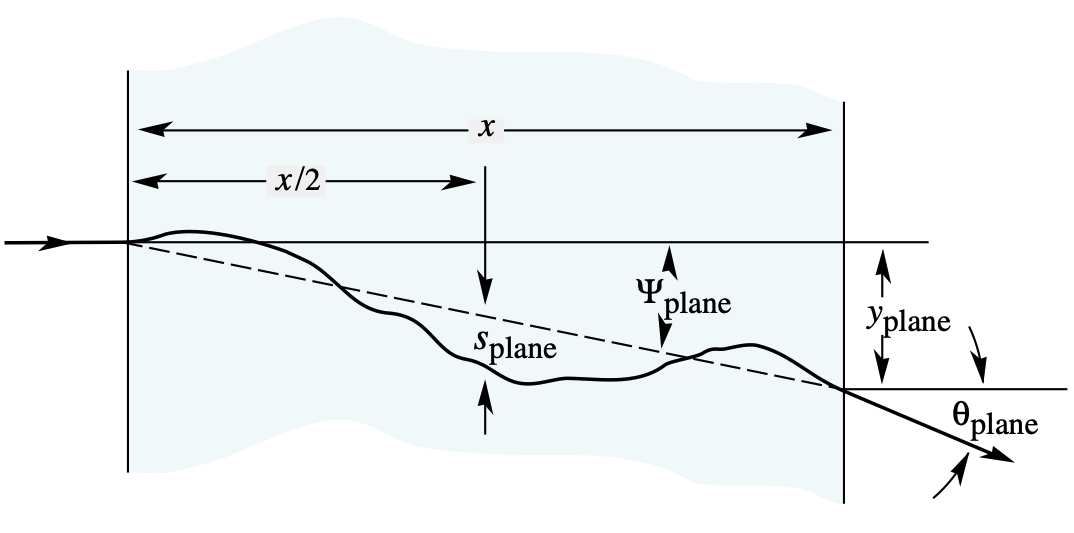
\includegraphics[width=0.65\linewidth]{figures/multi-scat.png}
    \caption{Schematic of the calculation of macroscopic mean deflection angle caused by multiple scattering~\cite{Zyla:2020zbs}.}
    \label{fig:multi-scat}
\end{figure}

The material effects described in this section, sections \ref{subsect:e-loss-heavy} and \ref{subsect:e-loss-electron}, are sufficient for Monte-Carlo simulations of the particle passage through material in the ITk. 
The overall trajectory can be discretized into small segments. 
The mean energy loss and Coulomb scattering angle over each segment can be estimated using equations \eqref{eq:6.1}, \eqref{eq:6.12}, \eqref{eq:6.15} and \eqref{eq:6.17}, along with the material distribution as shown in figure \ref{subfig:itk-rad-len}. The actual energy loss and scattering angle are then sampled from the corresponding distribution. 

\section{Simulated samples}
\label{sect:simulated-samples}
The development and evaluation of the new tracking algorithm in this thesis is carried out using a sample of simulated $pp\rightarrow t\bar{t}$ events at center-of-mass energy $\sqrt{s}=14$ TeV, with average pile-up ranging from 190 to 210.
The actual number of pile-up interactions in each event is randomly sampled from a Poisson distribution centred at the average pile-up. 
The hard-scattering event is generated using the \textsc{Powheg Box v2} \cite{Frixione:2002ik, Frixione:2007vw, Nason:2004rx, Alioli:2010xd} generator at next-to-leading order in QCD with the \textsc{NNPDF3.0nlo} \cite{Ball:2014uwa} Parton Distribution Functions (PDFs).
The $h_{\mathrm{damp}}$ parameter\footnote{ $h_{damp}$ is a resummation damping factor and one of the parameters that controls the matching of \textsc{Powheg} matrix elements to the parton shower and regulates the high-$p_T$ radiation against which the $t\bar{t}$ system recoils. } is fixed to $1.5m_{\mathrm{top}}$ \cite{ATL-PHYS-PUB-2016-020} and the top quark mass to $m_{\mathrm{top}} = 172.5$ GeV.
Parton shower and hadronization are modeled using \textsc{Pythia 8.230}\cite{Sjostrand:2014zea}, with the A14 set of tuned parameters \cite{ATL-PHYS-PUB-2014-021} and using the \textsc{NNPDF2.3lo} \cite{Ball:2012cx} set of PDFs.
A semi-leptonic final state, in which one of the two $W$-bosons descending from the top quarks decays to an electron or a muon, is enforced. 
The decay of bottom and charm hadrons are performed by \textsc{EvtGen 1.6.0}\cite{Lange:2001uf}.
The simulation described here follows the procedure detailed in reference~\cite{Aad_2025}.

To simulate the pile-up background, a large pool of soft minimum-bias interactions is generated. 
Each event is created by overlaying a number of min-bias sub-events on the hard-scattering sub-event, and then digitizing the detector response. 
A feature of MC simulation in ATLAS is that the pile-up sub-events are not uniquely generated for each events but randomly sampled from the common pool, resulting in a dataset whose events are guaranteed to feature different hard-scattering events, but may share a portion of their pile-up background. 
A dataset of 100000 $t\bar{t}$ events are simulated, from which a subset of 10000 events is identified to share no pile-up particles with the remaining 90000.
This subset is dedicated to machine learning training and performance evaluation.
The hard-scattering particles of the 90000 are used to train an algorithm to construct graphs from detector hits.

